% ============================================================
% Material Complementar — Resumo expandido GCV 2026
% Acompanha "Teste de contaminação em LLMs aplicados à ACV
% regionalizada do material particulado em produção leiteira"
% ============================================================

\documentclass[12pt,a4paper]{article}

\usepackage[a4paper,top=2.5cm,bottom=2.5cm,left=3cm,right=3cm]{geometry}
\usepackage[utf8]{inputenc}
\usepackage[T1]{fontenc}
\usepackage[brazil,english]{babel}
\usepackage{mathptmx}
\usepackage[scaled=.90]{helvet}
\usepackage{courier}
\usepackage{setspace}
\singlespacing
\setlength{\parindent}{1.25cm}
\setlength{\parskip}{0pt}

\usepackage{fancyhdr}
\pagestyle{fancy}
\fancyhf{}
\renewcommand{\headrulewidth}{0pt}
\fancyfoot[R]{S\thepage}

\usepackage{titlesec}
\titleformat{\section}{\normalfont\bfseries\uppercase}{\thesection}{1em}{}
\titleformat{\subsection}{\normalfont\bfseries\uppercase}{\thesubsection}{1em}{}
\titleformat{\subsubsection}{\normalfont\bfseries}{\thesubsubsection}{1em}{}
\titlespacing*{\section}{0pt}{1\baselineskip}{0.5\baselineskip}
\titlespacing*{\subsection}{0pt}{0.8\baselineskip}{0.4\baselineskip}
\titlespacing*{\subsubsection}{0pt}{0.6\baselineskip}{0.3\baselineskip}

\usepackage{caption}
\captionsetup{font={small},labelfont={bf},labelsep=endash,justification=centering,skip=4pt}

\usepackage{graphicx}
\usepackage{booktabs}
\usepackage{array}
\usepackage{tabularx}
\usepackage{longtable}
\usepackage{amsmath}
\usepackage{amssymb}
\usepackage{xurl}
\usepackage[hidelinks]{hyperref}
\usepackage{microtype}
\usepackage{xcolor}
\usepackage{listings}
\lstdefinestyle{prompt}{
  basicstyle=\ttfamily\scriptsize,
  breaklines=true,
  breakatwhitespace=true,
  columns=fullflexible,
  keepspaces=true,
  upquote=true,
  showstringspaces=false,
  frame=single,
  framesep=4pt,
  rulecolor=\color{black!20},
  backgroundcolor=\color{black!2},
  xleftmargin=0pt,
  xrightmargin=0pt,
  extendedchars=true,
  literate=
    {á}{{\'a}}1 {à}{{\`a}}1 {ã}{{\~a}}1 {â}{{\^a}}1 {ä}{{\"a}}1
    {é}{{\'e}}1 {ê}{{\^e}}1 {í}{{\'i}}1 {ó}{{\'o}}1 {ô}{{\^o}}1 {õ}{{\~o}}1
    {ú}{{\'u}}1 {ç}{{\c c}}1 {Á}{{\'A}}1 {À}{{\`A}}1 {Ã}{{\~A}}1 {Â}{{\^A}}1
    {É}{{\'E}}1 {Ê}{{\^E}}1 {Í}{{\'I}}1 {Ó}{{\'O}}1 {Ô}{{\^O}}1 {Õ}{{\~O}}1
    {Ú}{{\'U}}1 {Ç}{{\c C}}1 {º}{{\textordmasculine}}1 {ª}{{\textordfeminine}}1
    {₂}{{\textsubscript{2}}}1 {²}{{\textsuperscript{2}}}1
    {⁻}{{\textsuperscript{-}}}1 {×}{{$\times$}}1 {α}{{$\alpha$}}1 {μ}{{$\mu$}}1
    {–}{{--}}1 {—}{{---}}1 {≥}{{$\geq$}}1 {≤}{{$\leq$}}1
}
\sloppy

\begin{document}

\begin{center}
{\bfseries\uppercase{Material Complementar}}\\[4pt]
{\bfseries\uppercase{Teste de contaminação em LLMs aplicados à ACV regionalizada do material particulado em produção leiteira}}
\end{center}

\vspace{0.5\baselineskip}

\begin{flushright}
\small
Lucas Rover --- PPGSAU/UTFPR --- lucasrover@alunos.utfpr.edu.br\\
Yara de Souza Tadano --- PPGSAU/UTFPR --- yaratadano@utfpr.edu.br
\end{flushright}

\vspace{0.5\baselineskip}

Este material complementar acompanha o resumo expandido submetido ao 9º Congresso Brasileiro sobre Gestão do Ciclo de Vida (GCV 2026) e reúne, em formato auditável: (i) os prompts utilizados em português e inglês; (ii) o inventário pré-processado e os fatores de caracterização que alimentaram os prompts; (iii) tabelas detalhadas dos 480 outputs registrados; (iv) figuras adicionais; (v) parâmetros completos do desenho experimental e de reprodutibilidade. Todo o pipeline, dados brutos e código de análise estão em repositório público (\url{https://github.com/Roverlucas/ia-acv-gcv2026}).

\tableofcontents

% ============================================================
\section{Detalhamento metodológico}

\subsection{Versões dos modelos e parâmetros de chamada}

A Tabela~\ref{tab:sm_models} apresenta as versões exatas dos LLMs e os parâmetros de chamada utilizados em todas as 480 inferências registradas.

\begin{table}[h]
\centering
\small
\caption{Modelos LLM avaliados e parâmetros de chamada}
\label{tab:sm_models}
\begin{tabular}{lllc}
\toprule
\textbf{Provedor} & \textbf{Modelo} & \textbf{Versão da API} & \textbf{\emph{Seed} suportado} \\
\midrule
OpenAI    & GPT-4.1          & \texttt{gpt-4.1-2025-04-14} & 42 \\
Google    & Gemini 2.5 Pro   & \texttt{gemini-2.5-pro}     & Não suportado \\
DeepSeek  & DeepSeek V3      & \texttt{deepseek-chat}      & 42 \\
\bottomrule
\end{tabular}
\caption*{Fonte: autores. Temperatura fixada em 0 em todas as chamadas. \emph{Max output tokens}: 4096 (OpenAI, DeepSeek); 16\,384 (Gemini, devido ao uso interno de \emph{thinking tokens}). Formato de resposta forçado a JSON (\emph{response\_format}) em OpenAI e DeepSeek.}
\end{table}

\subsection{Esquema canônico da resposta JSON}

Todas as respostas exigidas em formato JSON estrito, validadas contra o esquema:

\begin{lstlisting}[style=prompt]
{
  "answer": {
    "global":   { "value": <numero ou null>, "unit": "DALY/kg FPCM" },
    "brazil":   { "value": <numero ou null>, "unit": "DALY/kg FPCM" },
    "state":    { "value": <numero ou null>, "unit": "DALY/kg FPCM" }
  },
  "characterization_model": "<modelo adotado>",
  "allocation_method": "<economic | mass | system_expansion | none | other | unspecified>",
  "reasoning": "<raciocinio passo a passo>",
  "intermediate_steps": [ { "step": "...", "value": <num>, "unit": "..." } ],
  "references": [ { "citation": "...", "doi": "..." } ],
  "uncertainties": "<o que nao foi possivel calcular>",
  "confidence": "<low | medium | high>"
}
\end{lstlisting}

\subsection{Critérios operacionais (recapitulação)}

\textbf{Concordância operacional.} Erro relativo absoluto $<30\%$ contra o \emph{ground truth} publicado.

\textbf{Classificação do teste de contaminação} (Seção~\ref{sec:stress}):
\begin{itemize}
\setlength\itemsep{0.2em}
\item \emph{Cálculo}: $|\Delta_{\text{novo}}|<10\%$ contra o novo GT calculado a partir do inventário perturbado.
\item \emph{Memorização}: $|\Delta_{\text{orig}}|<10\%$ contra o GT publicado em Giusti \emph{et al.} (2023).
\item \emph{Misto}: nenhum dos dois critérios é satisfeito.
\item \emph{Null}: o LLM recusa numericamente (retorna \texttt{null}).
\end{itemize}

% ============================================================
\section{Prompts utilizados (PT-BR e EN)}

Esta seção reproduz o texto integral dos prompts utilizados em todas as 480 chamadas. Os \emph{placeholders} \texttt{\{\{LCI\_TABLE\}\}}, \texttt{\{\{CF\_TABLE\_OBERSCHELP\}\}}, \texttt{\{\{STATE\_NAME\_PT\}\}}, \texttt{\{\{STATE\_NAME\_EN\}\}} e \texttt{\{\{STATE\_CODE\}\}} são substituídos automaticamente pelo orquestrador (\texttt{src/render\_prompt.py}) com os valores apropriados para cada sistema avaliado (S1: São Paulo/SP; S2: Paraná/PR).

\subsection{Instrução de sistema (PT-BR)}
\lstinputlisting[style=prompt]{supplementary/prompts/_system_instruction_pt.md}

\subsection{Instrução de sistema (EN)}
\lstinputlisting[style=prompt]{supplementary/prompts/_system_instruction_en.md}

\subsection{Nível L0 --- Zero context}
\subsubsection{Português}
\lstinputlisting[style=prompt]{supplementary/prompts/L0_zero_context_pt.md}
\subsubsection{Inglês}
\lstinputlisting[style=prompt]{supplementary/prompts/L0_zero_context_en.md}

\subsection{Nível L1 --- Scoped}
\subsubsection{Português}
\lstinputlisting[style=prompt]{supplementary/prompts/L1_scoped_pt.md}
\subsubsection{Inglês}
\lstinputlisting[style=prompt]{supplementary/prompts/L1_scoped_en.md}

\subsection{Nível L2 --- com LCI}
\subsubsection{Português}
\lstinputlisting[style=prompt]{supplementary/prompts/L2_with_lci_pt.md}
\subsubsection{Inglês}
\lstinputlisting[style=prompt]{supplementary/prompts/L2_with_lci_en.md}

\subsection{Nível L3 --- com fatores}
\subsubsection{Português}
\lstinputlisting[style=prompt]{supplementary/prompts/L3_with_factors_pt.md}
\subsubsection{Inglês}
\lstinputlisting[style=prompt]{supplementary/prompts/L3_with_factors_en.md}

\subsection{Nível L4 --- com procedimento}
\subsubsection{Português}
\lstinputlisting[style=prompt]{supplementary/prompts/L4_with_procedure_pt.md}
\subsubsection{Inglês}
\lstinputlisting[style=prompt]{supplementary/prompts/L4_with_procedure_en.md}

% ============================================================
\section{Dados pré-processados injetados nos prompts}

Esta seção reproduz os blocos de dados (inventários agregados e fatores de caracterização) substituídos nos \emph{placeholders} dos prompts L2--L4 para cada sistema. A reconciliação dos fatores nativos extraídos do material suplementar de Oberschelp \emph{et al.} (2020) com a planilha de cálculo de Giusti \emph{et al.} (2023) apresentou discrepância inferior a $0{,}1\%$.

\subsection{Sistema 1 --- inventário PM-relevante (alocação econômica)}
\lstinputlisting[style=prompt]{supplementary/data/s1_lci.md}

\subsection{Sistema 2 --- inventário PM-relevante (alocação econômica)}
\lstinputlisting[style=prompt]{supplementary/data/s2_lci.md}

\subsection{Sistema 1 --- fatores de caracterização Oberschelp (2020)}
\lstinputlisting[style=prompt]{supplementary/data/s1_cf.md}

\subsection{Sistema 2 --- fatores de caracterização Oberschelp (2020)}
\lstinputlisting[style=prompt]{supplementary/data/s2_cf.md}

% ============================================================
\section{Resultados completos do experimento principal}

\subsection{MAPE por (LLM $\times$ nível $\times$ idioma $\times$ escopo)}

\begin{table}[h]
\centering
\small
\caption{S1. Erro relativo absoluto m\'edio (MAPE) por (LLM $\times$ n\'ivel $\times$ idioma $\times$ escopo geogr\'afico) --- Sistema 1.}
\label{tab:sm_mape_s1}
\begin{tabular}{llccc}
\toprule
\textbf{LLM} & \textbf{Nivel / Idioma} & \textbf{Global} & \textbf{Brasil} & \textbf{Estado} \\
\midrule
GPT & L0 / pt-BR & $+5.0\times$ & $+1.1\times$ & +65\% \\
GPT & L0 / en & $+4.2\times$ & $+1.1\times$ & +83\% \\
GPT & L1 / pt-BR & $+7.8\times$ & $+1.9\times$ & +81\% \\
GPT & L1 / en & --- & --- & --- \\
GPT & L2 / pt-BR & --- & --- & --- \\
GPT & L2 / en & --- & --- & --- \\
GPT & L3 / pt-BR & +7\% & +24\% & +26\% \\
GPT & L3 / en & +9\% & +21\% & +23\% \\
GPT & L4 / pt-BR & +5\% & +16\% & +17\% \\
GPT & L4 / en & +9\% & +7\% & +7\% \\
\midrule
Gemini & L0 / pt-BR & $+8.3\times$ & $+3.2\times$ & --- \\
Gemini & L0 / en & $+33.5\times$ & $+14.9\times$ & $+2.2\times$ \\
Gemini & L1 / pt-BR & $+351.5\times$ & $+175.5\times$ & --- \\
Gemini & L1 / en & $+182.9\times$ & $+81.0\times$ & +48\% \\
Gemini & L2 / pt-BR & $+3.9\times$ & $+1.3\times$ & --- \\
Gemini & L2 / en & +75\% & +44\% & +93\% \\
Gemini & L3 / pt-BR & +3\% & +4\% & +4\% \\
Gemini & L3 / en & +0\% & +0\% & +0\% \\
Gemini & L4 / pt-BR & +0\% & +0\% & +0\% \\
Gemini & L4 / en & +0\% & +0\% & +0\% \\
\midrule
DeepSeek & L0 / pt-BR & $+4.3\times$ & $+1.5\times$ & +61\% \\
DeepSeek & L0 / en & $+41.4\times$ & $+17.5\times$ & $+1.8\times$ \\
DeepSeek & L1 / pt-BR & $+179.2\times$ & $+77.5\times$ & $+11.6\times$ \\
DeepSeek & L1 / en & $+41.4\times$ & $+17.5\times$ & $+1.8\times$ \\
DeepSeek & L2 / pt-BR & $+4.3\times$ & +85\% & +76\% \\
DeepSeek & L2 / en & $+4345.7\times$ & $+1516.1\times$ & $+192.0\times$ \\
DeepSeek & L3 / pt-BR & $+20.7\times$ & $+16.4\times$ & $+15.8\times$ \\
DeepSeek & L3 / en & +35\% & +7\% & +3\% \\
DeepSeek & L4 / pt-BR & +19\% & +19\% & +21\% \\
DeepSeek & L4 / en & +2\% & +4\% & +8\% \\
\bottomrule
\end{tabular}
\end{table}

\begin{table}[h]
\centering
\small
\caption{S2. Erro relativo absoluto m\'edio (MAPE) por (LLM $\times$ n\'ivel $\times$ idioma $\times$ escopo geogr\'afico) --- Sistema 2.}
\label{tab:sm_mape_s2}
\begin{tabular}{llccc}
\toprule
\textbf{LLM} & \textbf{Nivel / Idioma} & \textbf{Global} & \textbf{Brasil} & \textbf{Estado} \\
\midrule
GPT & L0 / pt-BR & $+15.4\times$ & +10\% & --- \\
GPT & L0 / en & $+18.5\times$ & $+1.6\times$ & --- \\
GPT & L1 / pt-BR & $+16.5\times$ & +93\% & --- \\
GPT & L1 / en & --- & --- & --- \\
GPT & L2 / pt-BR & --- & --- & --- \\
GPT & L2 / en & --- & --- & --- \\
GPT & L3 / pt-BR & +49\% & $+2.1\times$ & $+1.7\times$ \\
GPT & L3 / en & +69\% & +41\% & +13\% \\
GPT & L4 / pt-BR & +20\% & +76\% & +54\% \\
GPT & L4 / en & +17\% & +55\% & +35\% \\
\midrule
Gemini & L0 / pt-BR & $+91.9\times$ & $+10.5\times$ & --- \\
Gemini & L0 / en & $+128.5\times$ & $+15.5\times$ & $+12.5\times$ \\
Gemini & L1 / pt-BR & $+1611.0\times$ & $+7.9\times$ & --- \\
Gemini & L1 / en & $+1330.3\times$ & $+213.3\times$ & $+9.4\times$ \\
Gemini & L2 / pt-BR & $+1.5\times$ & +51\% & --- \\
Gemini & L2 / en & $+3.7\times$ & +75\% & +21\% \\
Gemini & L3 / pt-BR & +0\% & +0\% & +0\% \\
Gemini & L3 / en & +0\% & +0\% & +0\% \\
Gemini & L4 / pt-BR & +0\% & +0\% & +0\% \\
Gemini & L4 / en & +0\% & +0\% & +0\% \\
\midrule
DeepSeek & L0 / pt-BR & $+10.7\times$ & +83\% & +38\% \\
DeepSeek & L0 / en & $+92.7\times$ & $+12.7\times$ & $+10.6\times$ \\
DeepSeek & L1 / pt-BR & $+92.7\times$ & $+12.7\times$ & $+9.9\times$ \\
DeepSeek & L1 / en & $+116.1\times$ & $+17.3\times$ & $+15.1\times$ \\
DeepSeek & L2 / pt-BR & $+7494.7\times$ & $+875.5\times$ & $+617.1\times$ \\
DeepSeek & L2 / en & $+9599.9\times$ & $+1121.7\times$ & $+790.7\times$ \\
DeepSeek & L3 / pt-BR & $+1169.8\times$ & $+1167.3\times$ & $+1389.3\times$ \\
DeepSeek & L3 / en & +62\% & +20\% & +50\% \\
DeepSeek & L4 / pt-BR & +67\% & +25\% & +53\% \\
DeepSeek & L4 / en & +38\% & +17\% & +52\% \\
\bottomrule
\end{tabular}
\end{table}

\subsection{Curvas de saturação por sistema}

\begin{figure}[h]
\centering
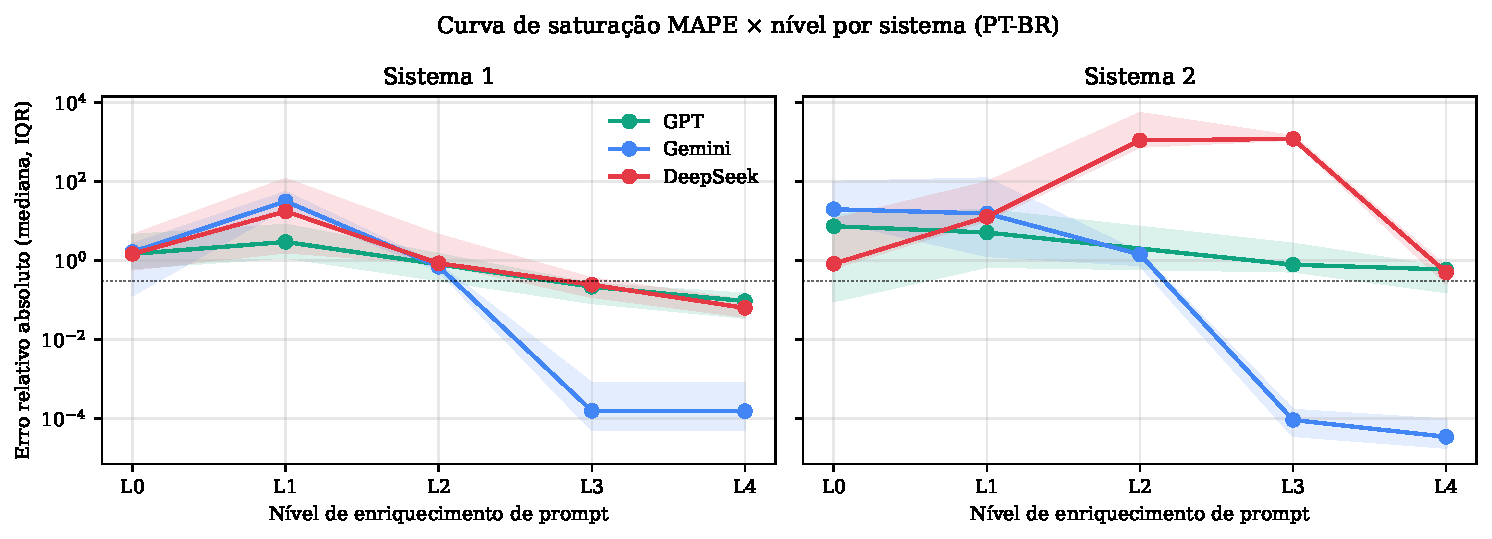
\includegraphics[width=\textwidth]{supplementary/figures/sm_fig1_mape_by_system.pdf}
\caption{Erro relativo absoluto (mediana, IQR) por nível de enriquecimento de prompt, separado por sistema (PT-BR). Eixo $y$ em escala logarítmica.}
\label{fig:sm_mape_sys}
\end{figure}

\subsection{Distribuição da log-razão}

\begin{figure}[h]
\centering
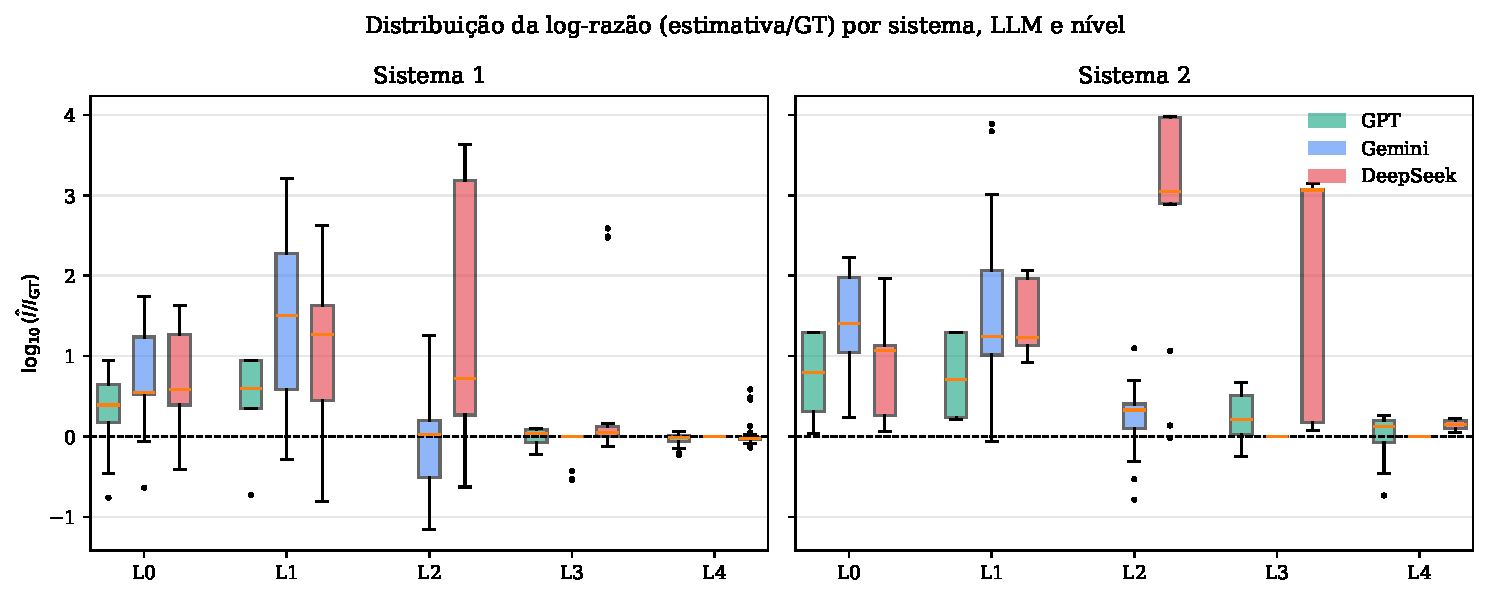
\includegraphics[width=\textwidth]{supplementary/figures/sm_fig2_log_ratio.pdf}
\caption{Distribuição do $\log_{10}(\hat{I}/I_{\mathrm{GT}})$ por sistema, LLM e nível.}
\label{fig:sm_logratio}
\end{figure}

\subsection{Coeficiente de variação intra-célula}

\begin{table}[h]
\centering
\small
\caption{Coeficiente de varia\c{c}\~ao intra-c\'elula (CV entre 5 repeti\c{c}\~oes), m\'edia sobre 3 escopos geogr\'aficos.}
\label{tab:sm_cv}
\begin{tabular}{cllcc}
\toprule
\textbf{Sis.} & \textbf{LLM} & \textbf{Nivel} & \textbf{CV (PT-BR)} & \textbf{CV (EN)} \\
\midrule
S1 & GPT & L0 & 0.126 & 0.379 \\
S1 & GPT & L1 & 0.097 & --- \\
S1 & GPT & L2 & --- & --- \\
S1 & GPT & L3 & 0.184 & 0.133 \\
S1 & GPT & L4 & 0.149 & 0.061 \\
S1 & Gemini & L0 & 1.504 & 0.409 \\
S1 & Gemini & L1 & 1.661 & 0.704 \\
S1 & Gemini & L2 & 1.449 & 0.236 \\
S1 & Gemini & L3 & 0.154 & 0.000 \\
S1 & Gemini & L4 & 0.000 & 0.000 \\
S1 & DeepSeek & L0 & 0.000 & 0.000 \\
S1 & DeepSeek & L1 & 1.110 & 0.000 \\
S1 & DeepSeek & L2 & 0.000 & 0.000 \\
S1 & DeepSeek & L3 & 3.984 & 0.021 \\
S1 & DeepSeek & L4 & 0.491 & 0.019 \\
\midrule
S2 & GPT & L0 & 0.048 & 0.000 \\
S2 & GPT & L1 & 0.235 & --- \\
S2 & GPT & L2 & --- & --- \\
S2 & GPT & L3 & 0.374 & 0.067 \\
S2 & GPT & L4 & 0.401 & 0.023 \\
S2 & Gemini & L0 & 0.483 & 0.606 \\
S2 & Gemini & L1 & 1.388 & 1.870 \\
S2 & Gemini & L2 & 0.271 & 0.928 \\
S2 & Gemini & L3 & 0.000 & 0.000 \\
S2 & Gemini & L4 & 0.000 & 0.000 \\
S2 & DeepSeek & L0 & 0.054 & 0.000 \\
S2 & DeepSeek & L1 & 0.039 & 0.000 \\
S2 & DeepSeek & L2 & 0.499 & 0.000 \\
S2 & DeepSeek & L3 & 0.023 & 0.004 \\
S2 & DeepSeek & L4 & 0.020 & 0.035 \\
\bottomrule
\end{tabular}
\end{table}

\begin{figure}[h]
\centering
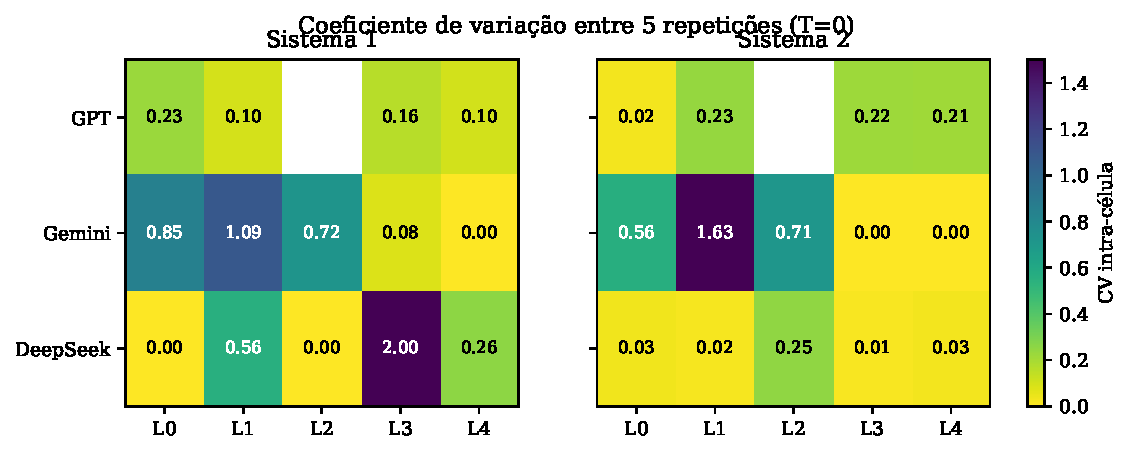
\includegraphics[width=\textwidth]{supplementary/figures/sm_fig4_cv_heatmap.pdf}
\caption{Coeficiente de variação intra-célula entre 5 repetições sob $T=0$, média sobre 3 escopos geográficos e 2 idiomas.}
\label{fig:sm_cv}
\end{figure}

\subsection{Modelo de caracterização declarado pelos LLMs}

\begin{table}[h]
\centering
\small
\caption{Modelo de caracteriza\c{c}\~ao declarado pelos LLMs por (sistema $\times$ n\'ivel). Conta-se PT-BR + EN.}
\label{tab:sm_char_choice}
\begin{tabular}{clccccc}
\toprule
\textbf{Sis.} & \textbf{Nivel} & \textbf{Oberschelp} & \textbf{ReCiPe 2016} & \textbf{IMPACT World+} & \textbf{Outro} & \textbf{N\~ao espec.} \\
\midrule
S1 & L0 & 0 & 14 & 16 & 0 & 0 \\
S1 & L1 & 0 & 13 & 12 & 0 & 5 \\
S1 & L2 & 0 & 10 & 9 & 10 & 1 \\
S1 & L3 & 29 & 0 & 0 & 0 & 1 \\
S1 & L4 & 30 & 0 & 0 & 0 & 0 \\
\midrule
S2 & L0 & 0 & 17 & 13 & 0 & 0 \\
S2 & L1 & 0 & 12 & 13 & 0 & 5 \\
S2 & L2 & 0 & 8 & 12 & 9 & 1 \\
S2 & L3 & 29 & 0 & 0 & 0 & 1 \\
S2 & L4 & 29 & 0 & 0 & 0 & 1 \\
\bottomrule
\end{tabular}
\end{table}

% ============================================================
\section{Teste de contaminação --- detalhado}
\label{sec:stress}

\subsection{Esquemas de perturbação}

\begin{description}
\setlength\itemsep{0.2em}
\item[P1 (escala uniforme):] todas as massas de emissão multiplicadas por $2{,}0$. Novo \emph{ground truth} esperado $= 2\times$ original.
\item[P2 (amônia atenuada):] massa de amônia (NH$_3$, precursor dominante para PM secundário) multiplicada por $0{,}1$, demais inalteradas. Para o Sistema 1, novo GT esperado $\approx 0{,}37\times$ original; para o Sistema 2, $\approx 0{,}57\times$.
\item[P3 (perturbação aleatória):] cada substância multiplicada por um fator aleatório $\sim$U[0,5;\,2,0] com \emph{seed} fixa (42), produzindo um novo GT determinístico mas sem padrão geométrico imediato.
\end{description}

Em todas as 180 chamadas do teste, o prompt inclui nota experimental explícita informando que o inventário é hipotético e instruindo cálculo estrito sobre os números fornecidos.

\subsection{Classificação por (sistema $\times$ LLM $\times$ esquema $\times$ nível)}

\begin{table}[h]
\centering
\small
\caption{Classifica\c{c}\~ao detalhada das 180 chamadas do teste de contamina\c{c}\~ao por (sistema $\times$ LLM $\times$ esquema $\times$ n\'ivel). Cada c\'elula tem $n=5$ chamadas.}
\label{tab:sm_stress_detail}
\begin{tabular}{ccllcccc}
\toprule
\textbf{Sis.} & \textbf{LLM} & \textbf{Esquema} & \textbf{Nivel} & \textbf{C\'alc.} & \textbf{Mem.} & \textbf{Misto} & \textbf{Null} \\
\midrule
S1 & GPT & P1 & L3 & 0 & 5 & 0 & 0 \\
S1 & GPT & P1 & L4 & 0 & 5 & 0 & 0 \\
S1 & GPT & P2 & L3 & 0 & 5 & 0 & 0 \\
S1 & GPT & P2 & L4 & 0 & 2 & 3 & 0 \\
S1 & GPT & P3 & L3 & 0 & 5 & 0 & 0 \\
S1 & GPT & P3 & L4 & 0 & 5 & 0 & 0 \\
\midrule
S1 & Gemini & P1 & L3 & 0 & 5 & 0 & 0 \\
S1 & Gemini & P1 & L4 & 0 & 5 & 0 & 0 \\
S1 & Gemini & P2 & L3 & 1 & 4 & 0 & 0 \\
S1 & Gemini & P2 & L4 & 0 & 5 & 0 & 0 \\
S1 & Gemini & P3 & L3 & 0 & 5 & 0 & 0 \\
S1 & Gemini & P3 & L4 & 0 & 5 & 0 & 0 \\
\midrule
S1 & DeepSeek & P1 & L3 & 0 & 1 & 4 & 0 \\
S1 & DeepSeek & P1 & L4 & 0 & 4 & 1 & 0 \\
S1 & DeepSeek & P2 & L3 & 0 & 0 & 5 & 0 \\
S1 & DeepSeek & P2 & L4 & 0 & 4 & 0 & 1 \\
S1 & DeepSeek & P3 & L3 & 1 & 0 & 4 & 0 \\
S1 & DeepSeek & P3 & L4 & 0 & 4 & 1 & 0 \\
\midrule
S2 & GPT & P1 & L3 & 0 & 0 & 5 & 0 \\
S2 & GPT & P1 & L4 & 0 & 0 & 5 & 0 \\
S2 & GPT & P2 & L3 & 0 & 0 & 5 & 0 \\
S2 & GPT & P2 & L4 & 0 & 0 & 5 & 0 \\
S2 & GPT & P3 & L3 & 0 & 3 & 2 & 0 \\
S2 & GPT & P3 & L4 & 0 & 0 & 5 & 0 \\
\midrule
S2 & Gemini & P1 & L3 & 0 & 5 & 0 & 0 \\
S2 & Gemini & P1 & L4 & 0 & 5 & 0 & 0 \\
S2 & Gemini & P2 & L3 & 0 & 5 & 0 & 0 \\
S2 & Gemini & P2 & L4 & 0 & 5 & 0 & 0 \\
S2 & Gemini & P3 & L3 & 0 & 5 & 0 & 0 \\
S2 & Gemini & P3 & L4 & 1 & 4 & 0 & 0 \\
\midrule
S2 & DeepSeek & P1 & L3 & 0 & 0 & 4 & 1 \\
S2 & DeepSeek & P1 & L4 & 0 & 0 & 5 & 0 \\
S2 & DeepSeek & P2 & L3 & 0 & 0 & 5 & 0 \\
S2 & DeepSeek & P2 & L4 & 0 & 0 & 5 & 0 \\
S2 & DeepSeek & P3 & L3 & 0 & 0 & 1 & 4 \\
S2 & DeepSeek & P3 & L4 & 4 & 0 & 1 & 0 \\
\bottomrule
\end{tabular}
\end{table}

\subsection{Resposta do LLM vs. novo \emph{ground truth}}

\begin{figure}[h]
\centering
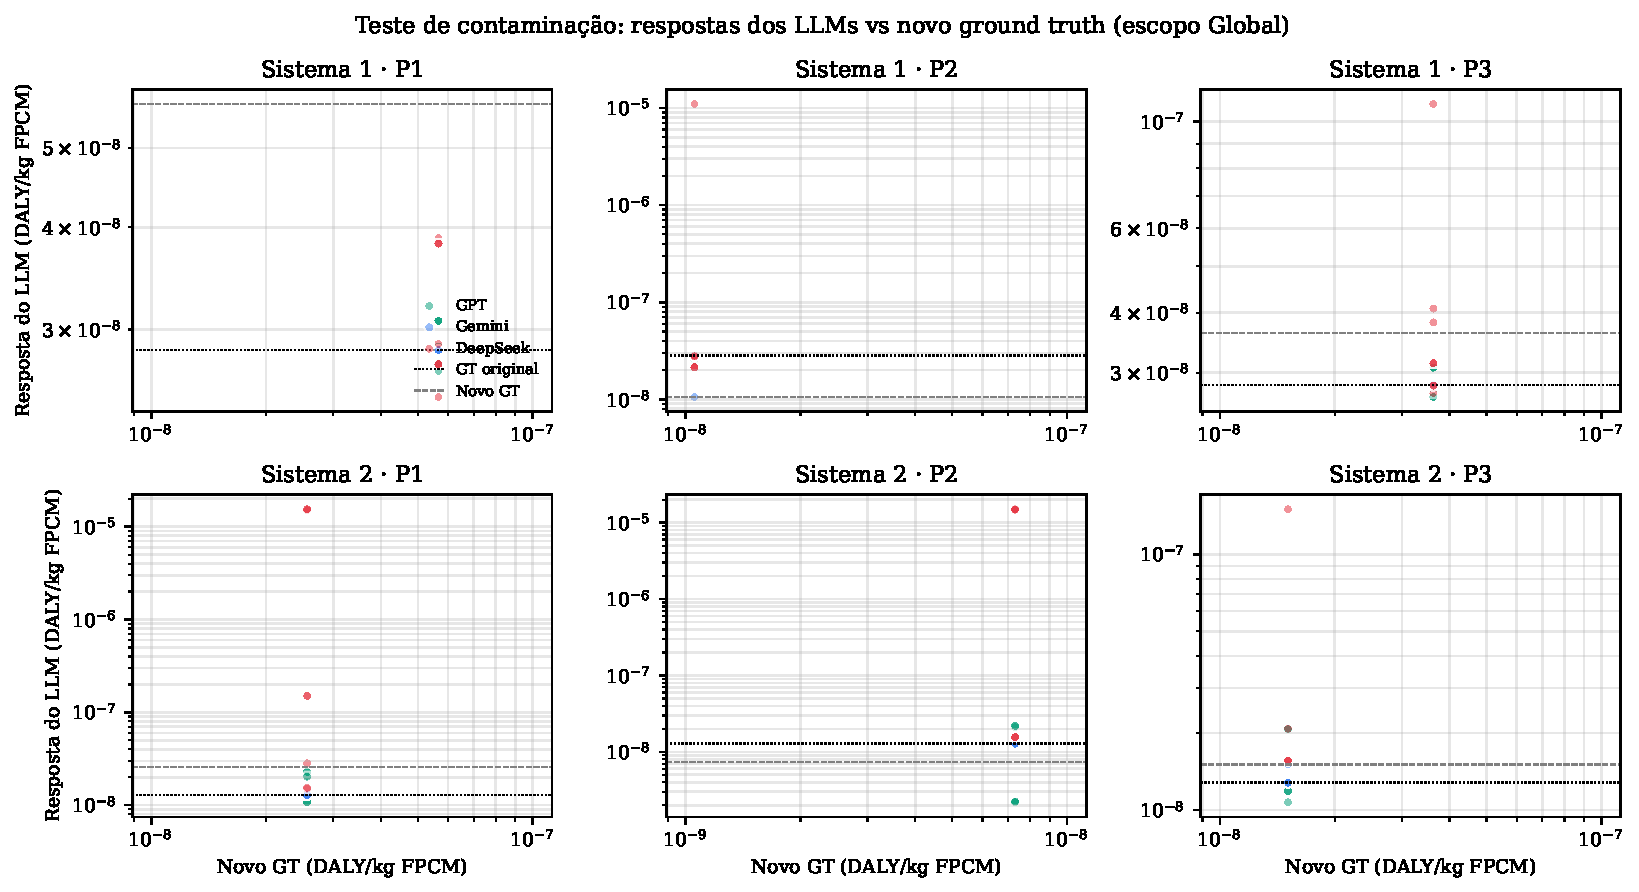
\includegraphics[width=\textwidth]{supplementary/figures/sm_fig3_stress_scatter.pdf}
\caption{Resposta do LLM (escopo Global) vs. novo \emph{ground truth} calculado para cada esquema de perturbação. Linha pontilhada: GT original publicado. Linha tracejada: novo GT esperado caso o LLM tivesse calculado a partir do inventário perturbado.}
\label{fig:sm_scatter}
\end{figure}

% ============================================================
\section{Comparação com o paper-referência}

\subsection{Tabela comparativa Giusti vs. LLMs}

A Tabela~\ref{tab:sm_comparative} apresenta lado a lado o \emph{ground truth} de GIUSTI \emph{et al.} (2023) e as medianas das respostas dos três LLMs nos níveis L3 e L4 (PT-BR, $n=10$ por célula). A Figura~\ref{fig:sm_giusti} apresenta a comparação visual em escala logarítmica.

\begin{table}[h]
\centering
\footnotesize
\caption{Comparação entre o \emph{ground truth} de Giusti \emph{et al.} (2023) e a mediana das respostas dos LLMs em L3+L4 (PT-BR, $n=10$ por célula). Valores em DALY/kg FPCM.}
\label{tab:sm_comparative}
\begin{tabular}{l l c c c}
\toprule
\textbf{Sistema} & \textbf{LLM / fonte} & \textbf{Global} & \textbf{Brasil} & \textbf{Estado} \\
\midrule
S1 (SP) & \textit{Giusti et al. (2023)} & $2.83 \times 10^{-8}$ & $8.11 \times 10^{-8}$ & $6.37 \times 10^{-7}$ \\
 & GPT-4.1 & $2.86 \times 10^{-8}$ & $8.29 \times 10^{-8}$ & $6.60 \times 10^{-7}$ \\
 & Gemini 2.5 Pro & $2.83 \times 10^{-8}$ & $8.10 \times 10^{-8}$ & $6.37 \times 10^{-7}$ \\
 & DeepSeek V3 & $2.82 \times 10^{-8}$ & $7.68 \times 10^{-8}$ & $5.82 \times 10^{-7}$ \\
\midrule
S2 (PR) & \textit{Giusti et al. (2023)} & $1.28 \times 10^{-8}$ & $1.10 \times 10^{-7}$ & $1.55 \times 10^{-7}$ \\
 & GPT-4.1 & $1.07 \times 10^{-8}$ & $2.02 \times 10^{-7}$ & $2.49 \times 10^{-7}$ \\
 & Gemini 2.5 Pro & $1.28 \times 10^{-8}$ & $1.10 \times 10^{-7}$ & $1.55 \times 10^{-7}$ \\
 & DeepSeek V3 & $7.51 \times 10^{-6}$ & $6.01 \times 10^{-5}$ & $1.00 \times 10^{-4}$ \\
\bottomrule
\end{tabular}
\end{table}

\begin{figure}[h]
\centering
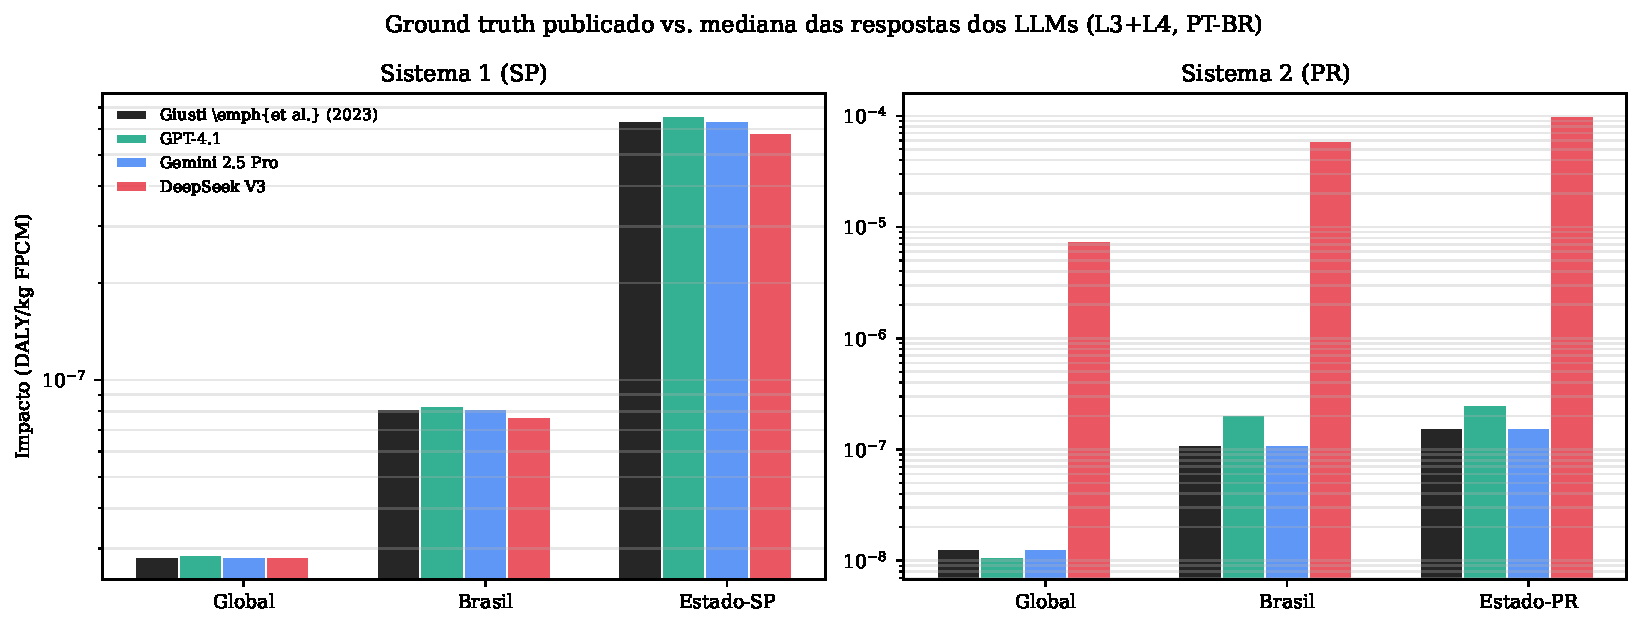
\includegraphics[width=\textwidth]{supplementary/figures/sm_fig5_giusti_vs_llm.pdf}
\caption{Ground truth publicado vs. mediana das respostas dos LLMs em L3+L4 (PT-BR). Eixo $y$ em escala logarítmica.}
\label{fig:sm_giusti}
\end{figure}

\subsection{Análise de sensibilidade ao limiar de classificação}

A classificação \emph{cálculo}/\emph{memorização}/\emph{misto} usa um limiar de $\pm 10\%$ contra os \emph{ground truths}. A Tabela~\ref{tab:sm_threshold} mostra que o ordenamento das taxas e a magnitude da diferença entre Gemini, GPT e DeepSeek são robustos sob limiares de $\pm 5\%$ e $\pm 15\%$.

\begin{table}[h]
\centering
\footnotesize
\caption{Sensibilidade da classificação à escolha do limiar (taxa de \emph{memorização} em \% para diferentes janelas).}
\label{tab:sm_threshold}
\begin{tabular}{l c ccc ccc}
\toprule
& & \multicolumn{3}{c}{\textbf{Sistema 1}} & \multicolumn{3}{c}{\textbf{Sistema 2}} \\
\textbf{LLM} & $n$ & 5\% & 10\% & 15\% & 5\% & 10\% & 15\% \\
\midrule
GPT-4.1 & 30 & 43\% & 90\% & 100\% & 0\% & 10\% & 10\% \\
Gemini 2.5 Pro & 30 & 97\% & 97\% & 97\% & 97\% & 97\% & 97\% \\
DeepSeek V3 & 30 & 45\% & 45\% & 59\% & 0\% & 0\% & 0\% \\
\bottomrule
\end{tabular}
\end{table}

\subsection{Decomposição da memorização por perturbação e por nível}

A Tabela~\ref{tab:sm_stress_break} apresenta a contagem de chamadas classificadas como \emph{memorização} estratificada por esquema de perturbação (P1, P2, P3) e por nível de prompt (L3, L4), revelando que o padrão é estável dentro de cada combinação LLM $\times$ sistema.

\begin{table}[h]
\centering
\footnotesize
\caption{Decomposição da taxa de \emph{memorização} por perturbação e por nível (chamadas/$5$ por célula).}
\label{tab:sm_stress_break}
\begin{tabular}{l l ccc ccc}
\toprule
& & \multicolumn{3}{c}{\textbf{L3}} & \multicolumn{3}{c}{\textbf{L4}} \\
\textbf{LLM} & \textbf{Sis.} & P1 & P2 & P3 & P1 & P2 & P3 \\
\midrule
GPT-4.1 & S1 & 5/5 & 5/5 & 5/5 & 5/5 & 2/5 & 5/5 \\
GPT-4.1 & S2 & 0/5 & 0/5 & 3/5 & 0/5 & 0/5 & 0/5 \\
Gemini 2.5 Pro & S1 & 5/5 & 4/5 & 5/5 & 5/5 & 5/5 & 5/5 \\
Gemini 2.5 Pro & S2 & 5/5 & 5/5 & 5/5 & 5/5 & 5/5 & 4/5 \\
DeepSeek V3 & S1 & 1/5 & 0/5 & 0/5 & 4/5 & 4/5 & 4/5 \\
DeepSeek V3 & S2 & 0/5 & 0/5 & 0/5 & 0/5 & 0/5 & 0/5 \\
\bottomrule
\end{tabular}
\end{table}

% ============================================================
\section{Diferenciação regional}

A razão \emph{Estado/Global} esperada é $22{,}5\times$ para o Sistema 1 e $12{,}1\times$ para o Sistema 2. Em L0--L2, os três LLMs reportam razões de $1{,}0\times$ a $3{,}0\times$, subestimando a diferenciação em uma a duas ordens de magnitude. A Tabela~\ref{tab:sm_regional} apresenta as razões medianas por (sistema $\times$ LLM $\times$ nível).

\begin{table}[h]
\centering
\small
\caption{Raz\~ao mediana \emph{Estado/Global} reportada pelos LLMs vs. \emph{ground truth} publicado.}
\label{tab:sm_regional}
\begin{tabular}{clccccc l}
\toprule
\textbf{Sis.} & \textbf{LLM} & \textbf{L0} & \textbf{L1} & \textbf{L2} & \textbf{L3} & \textbf{L4} & \textbf{GT publicado} \\
\midrule
S1 & GPT & 1.47 & 0.48 & --- & 21.65 & 22.41 & 22.52 \\
S1 & Gemini & 1.87 & 3.05 & 1.13 & 22.52 & 22.52 & 22.52 \\
S1 & DeepSeek & 1.58 & 1.50 & 1.00 & 17.45 & 20.21 & 22.52 \\
\midrule
S2 & GPT & --- & --- & --- & 15.79 & 19.78 & 12.13 \\
S2 & Gemini & 1.23 & 1.08 & 1.17 & 12.13 & 12.13 & 12.13 \\
S2 & DeepSeek & 1.50 & 1.58 & 1.00 & 13.33 & 11.96 & 12.13 \\
\bottomrule
\end{tabular}
\end{table}

% ============================================================
\section{Reprodutibilidade}

\subsection{Repositório público}

Todo o pipeline experimental, dados brutos (JSONL com as 480 chamadas), prompts versionados, scripts de análise e código LaTeX são disponibilizados em:

\begin{center}
\url{https://github.com/Roverlucas/ia-acv-gcv2026}
\end{center}

\subsection{Estrutura do repositório}

\begin{description}
\setlength\itemsep{0.2em}
\item[\texttt{prompts/templates/}] templates L0--L4 em PT-BR e EN, com instrução de sistema e esquema JSON.
\item[\texttt{prompts/runs/}] \emph{snapshot} dos prompts efetivamente executados (hash em SHA-256 truncado em 12 caracteres por arquivo).
\item[\texttt{src/run\_experiment.py}, \texttt{src/run\_stress\_test.py}] orquestradores das 300 chamadas do experimento principal e 180 do teste de contaminação.
\item[\texttt{src/analyze.py}, \texttt{src/analyze\_regional.py}, \texttt{src/figures.py}, \texttt{src/generate\_sm\_tables.py}, \texttt{src/generate\_sm\_figures.py}] pipeline de análise e geração de artefatos.
\item[\texttt{results/raw/*.jsonl}] respostas brutas das LLMs (480 linhas no total, em 6 arquivos JSONL).
\item[\texttt{data/processed/s\{1,2\}/}] inventários agregados, fatores de caracterização e \emph{ground truth} por sistema; inclui o subdiretório \texttt{stress/} com os inventários perturbados.
\item[\texttt{manuscript/gcv2026/}] resumo expandido e este material complementar em LaTeX.
\end{description}

\subsection{Conformidade de \emph{schema} JSON}

Das 480 chamadas registradas, 472 retornaram JSON conforme o esquema canônico em uma única tentativa; 8 falhas de \emph{parsing} (todas em DeepSeek L4 EN) foram recuperáveis por avaliação aritmética das expressões fornecidas em vez de literais numéricos no campo \texttt{value}. Nenhuma chamada exigiu reexecução.

\subsection{Custo agregado}

\begin{description}
\setlength\itemsep{0.2em}
\item[Experimento principal (300 chamadas):] US\$\,3{,}42, 108 minutos.
\item[Teste de contaminação (180 chamadas):] US\$\,2{,}65, $\approx 90$ minutos.
\item[\textbf{Total}] US\$\,6{,}07, $\approx 200$ minutos de execução.
\end{description}

\subsection{Conflito de interesse}

Uma das autoras (Yara de Souza Tadano) é coautora do paper-referência (Giusti \emph{et al.}, 2023). Toda comparação foi feita contra os números publicados, sem reanálise privilegiada do dado bruto.

\end{document}
